\documentclass[12pt,a4paper,oneside]{book}

% Bộ mã và tiếng Việt
\usepackage[utf8]{inputenc}
\usepackage[utf8]{vietnam}
\usepackage[T5]{fontenc}

% Các gói toán học và định dạng
\usepackage{amsmath, amssymb, amsfonts}
\usepackage{tipa}
\usepackage{booktabs}
\usepackage{mathptmx}

% Hình ảnh và bảng
\usepackage{graphicx}
\usepackage{subcaption}
\usepackage{float}
\usepackage{array}
\usepackage{multirow}
\usepackage{fancyhdr}
\graphicspath{{figs/}}

% Định nghĩa cột bảng có căn giữa
\newcolumntype{P}[1]{>{\centering\arraybackslash}p{#1}}
\newcolumntype{M}[1]{>{\centering\arraybackslash}m{#1}}

% Giải thuật
\usepackage{algorithm}
\usepackage{algpseudocode}
\makeatletter
\renewcommand{\ALG@name}{Giải thuật}
\renewcommand{\listalgorithmname}{Danh sách giải thuật}
\makeatother
\captionsetup[algorithm]{labelsep=colon}
\def\algbackskip{\hskip-\ALG@thistlm}

% Canh lề trang chuyên nghiệp
\usepackage[a4paper, top=2.5cm, bottom=2.5cm, left=3cm, right=3cm]{geometry}

% Font và dòng
\linespread{1.25}
\usepackage[skip=10pt plus1pt, indent=0pt]{parskip} % Không thụt đầu dòng

% Tô màu và liên kết
\usepackage[usenames,dvipsnames]{xcolor}
\definecolor{cobalt}{rgb}{0.0, 0.28, 0.67}
\definecolor{carmine}{rgb}{0.59, 0.0, 0.09}
\usepackage[unicode, colorlinks=true, urlcolor=carmine, citecolor=cobalt, linkcolor=carmine, pdfborder={0 0 0}]{hyperref}

% Loại bỏ trang trắng đầu tiên
\usepackage{atbegshi}
\AtBeginDocument{\AtBeginShipoutNext{\AtBeginShipoutDiscard}}


% Gói thesis riêng của template
\usepackage{styles/thesis}

% Đánh số tối đa tới subsubsection
\setcounter{secnumdepth}{2}

\usepackage{listings}  % hỗ trợ lstlisting


\thesislayout
\begin{document}

% Bìa báo cáo (SV sử dụng MS Word tạo bìa, sau đó export thành file PDF để ghép vào báo cáo)

\begin{titlepage}
\centering
\coverpage
\end{titlepage}


% --- Phần đầu tài liệu (roman numbering, không đánh số chapter) ---
\frontmatter

% --- Lời cảm ơn ---
\begin{acknowledgments}
Chúng em xin gửi lời cảm ơn chân thành đến Thầy/Cô đã tận tình giảng dạy và hỗ trợ trong suốt quá trình học tập. Đây là nền tảng vững chắc để chúng em thực hiện và hoàn thành bài tập lớn học phần "Nhập môn An toàn bảo mật thông tin".
\end{acknowledgments}

% --- Mục lục tự động ---
\tableofcontents
\listoffigures
\listoftables
\listofalgorithms  % Chỉ mở nếu có dùng gói thuật toán

% --- Phần nội dung chính ---
\mainmatter
\fancyhead{}
\renewcommand{\footrulewidth}{0.4pt}
\pagestyle{fancy} 
\renewcommand{\chaptermark}[1]{\markboth{#1}{#1}}
\fancyhead[R]{\chaptername\ \thechapter\ --\ \leftmark}

% --- Gọi các chương ---
\chapter{Giới thiệu}

\section{Bối cảnh và lý do chọn đề tài}

Trong thời đại công nghệ số, bảo mật thông tin tài chính là một yêu cầu then chốt đối với mọi tổ chức. Việc truyền tải báo cáo tài chính qua môi trường mạng tiềm ẩn nhiều nguy cơ bị đánh cắp, rò rỉ hoặc bị chỉnh sửa nội dung. Do đó, nhu cầu phát triển một hệ thống giúp đảm bảo tính bảo mật, toàn vẹn và hiệu quả truyền tải dữ liệu là hết sức cần thiết.

Đề tài “Gửi báo cáo tài chính có nén và mã hóa” được lựa chọn với mục tiêu giải quyết bài toán trên bằng cách áp dụng kết hợp giữa các kỹ thuật nén dữ liệu và mã hóa đối xứng. Dữ liệu sẽ được nén nhằm giảm kích thước truyền tải, sau đó được mã hóa để đảm bảo tính bảo mật, trước khi được truyền từ máy khách (client) đến máy chủ (server).

\section{Mục tiêu của đề tài}

Đề tài hướng đến việc xây dựng một hệ thống có các chức năng chính sau:

\begin{itemize}
  \item Nén tệp báo cáo tài chính đầu vào nhằm tối ưu hóa dung lượng truyền tải.
  \item Mã hóa tệp nén sử dụng kỹ thuật mã hóa đối xứng (AES hoặc tương đương).
  \item Gửi dữ liệu đã mã hóa thông qua kết nối mạng socket TCP.
  \item Tại phía máy chủ, giải mã và giải nén để phục hồi tệp gốc.
  \item Đảm bảo tính toàn vẹn và bảo mật trong toàn bộ quá trình truyền dữ liệu.
\end{itemize}

\section{Phạm vi và ứng dụng thực tế}

Phạm vi của đề tài giới hạn ở mức truyền một tệp báo cáo tài chính định dạng PDF giữa một client và một server trong mạng nội bộ. Tuy nhiên, hệ thống có thể dễ dàng mở rộng để áp dụng trong các môi trường lớn hơn như:
Nội dung hệ thống sử dụng mã hóa đối xứng DES \cite{desAlgorithm} và socket trong Python \cite{pythonSocket}.

\begin{itemize}
  \item Truyền tài liệu giữa các chi nhánh ngân hàng.
  \item Giao tiếp an toàn giữa các phòng ban trong doanh nghiệp.
  \item Nền tảng cơ bản cho các ứng dụng truyền dữ liệu bảo mật qua mạng Internet.
\end{itemize}

Thông qua đề tài, sinh viên có cơ hội tiếp cận với các kỹ thuật nén và mã hóa cơ bản, đồng thời thực hành lập trình socket, một kỹ năng quan trọng trong lĩnh vực bảo mật và mạng máy tính.


\chapter{Cơ sở lý thuyết}

\section{Nén dữ liệu}

Nén dữ liệu là quá trình giảm kích thước tệp tin bằng cách loại bỏ các dữ liệu dư thừa hoặc biểu diễn dữ liệu theo cách tối ưu hơn. Quá trình này giúp tiết kiệm băng thông khi truyền tải qua mạng, đồng thời rút ngắn thời gian gửi và nhận. Trong phạm vi đề tài, thuật toán nén ZIP được sử dụng vì tính phổ biến, hiệu quả và dễ tích hợp với ngôn ngữ lập trình Python thông qua thư viện \texttt{zipfile}.

Nén không làm thay đổi nội dung dữ liệu gốc và có thể phục hồi chính xác 100\% sau khi giải nén, do đó phù hợp để truyền tải các tài liệu tài chính quan trọng.

\section{Mã hóa đối xứng}

Mã hóa là quá trình chuyển đổi dữ liệu từ dạng có thể đọc được (plaintext) sang dạng không thể đọc được (ciphertext), nhằm đảm bảo rằng chỉ người được cấp quyền mới có thể truy cập thông tin gốc. Trong đề tài này, mã hóa đối xứng được sử dụng, cụ thể là thuật toán AES (Advanced Encryption Standard).

AES là thuật toán mã hóa khối, sử dụng cùng một khóa cho cả mã hóa và giải mã. Nó được tiêu chuẩn hóa bởi NIST và sử dụng rộng rãi trong nhiều hệ thống bảo mật thực tế vì có tốc độ cao, mức độ bảo mật mạnh và dễ triển khai. Việc kết hợp mã hóa với nén giúp nâng cao cả tính bảo mật lẫn hiệu suất truyền tải.

\section{Lập trình socket trong Python}

Socket là một giao diện lập trình mạng cho phép hai thiết bị giao tiếp với nhau thông qua các giao thức như TCP hoặc UDP. Trong đề tài này, giao thức TCP được sử dụng để đảm bảo việc truyền dữ liệu diễn ra đáng tin cậy, đúng thứ tự và không mất mát.

Python cung cấp mô-đun \texttt{socket}, cho phép lập trình viên dễ dàng xây dựng các ứng dụng mạng dạng client-server. Mô hình truyền tải trong hệ thống đề xuất bao gồm một máy khách gửi tệp nén và mã hóa qua socket tới máy chủ, nơi dữ liệu sẽ được giải mã và giải nén.

\section{Tính toàn vẹn và bảo mật trong truyền dữ liệu}

Bảo mật không chỉ bao gồm việc giữ kín nội dung (confidentiality), mà còn phải đảm bảo tính toàn vẹn (integrity) và xác thực (authenticity) của dữ liệu. Trong đề tài, tính toàn vẹn được đảm bảo bằng cách kiểm tra sự khớp nhau giữa dữ liệu trước và sau quá trình nhận. Ngoài ra, việc sử dụng khóa mã hóa riêng giữa client và server giúp ngăn chặn truy cập trái phép.

\section{Thư viện sử dụng}

Trong quá trình hiện thực đề tài, các thư viện Python sau được sử dụng:

\begin{itemize}
  \item \textbf{zipfile}: nén và giải nén dữ liệu theo định dạng ZIP.
  \item \textbf{cryptography.fernet}: mã hóa và giải mã dữ liệu bằng khóa đối xứng an toàn.
  \item \textbf{socket}: lập trình mạng giữa client và server.
  \item \textbf{os, sys}: thao tác với hệ thống tệp và xử lý tham số dòng lệnh.
\end{itemize}

Những thư viện này giúp đơn giản hóa quá trình lập trình, đảm bảo hiệu quả triển khai và dễ bảo trì hệ thống.

\chapter{Thiết kế và Cài đặt}

\section{Kiến trúc tổng thể của hệ thống}

Hệ thống được thiết kế theo mô hình client–server với hai thành phần chính:

\begin{itemize}
  \item \textbf{Client}: thực hiện nén tệp, mã hóa và gửi dữ liệu.
  \item \textbf{Server}: nhận dữ liệu, giải mã và giải nén để khôi phục tệp gốc.
\end{itemize}

Quá trình truyền dữ liệu đảm bảo tính bảo mật và toàn vẹn nhờ áp dụng kết hợp kỹ thuật mã hóa đối xứng và nén tệp. Hình \ref{fig:system_architecture} minh họa kiến trúc tổng thể của hệ thống.

\begin{figure}[H]
  \centering
  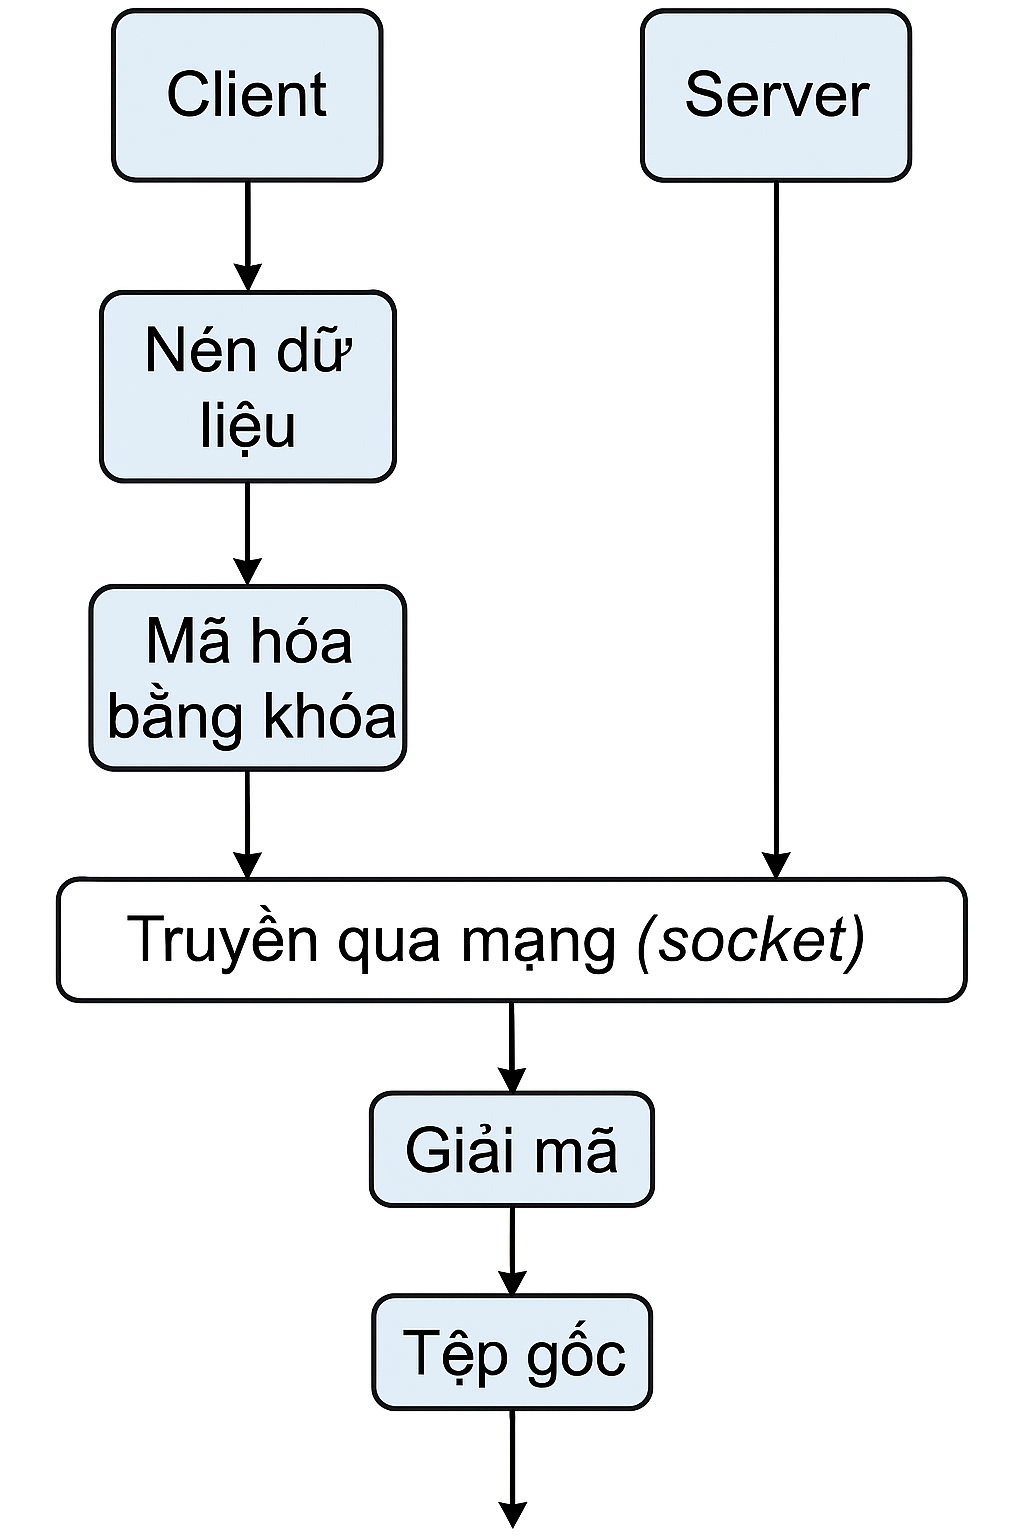
\includegraphics[width=0.95\textwidth]{figs/architecture.png}
  \caption{Kiến trúc hệ thống gửi báo cáo tài chính}
  \label{fig:system_architecture}
\end{figure}

\section{Quy trình xử lý tại phía Client}

Các bước xử lý tại máy khách bao gồm:

\begin{enumerate}
  \item Chọn tệp đầu vào (ví dụ: \texttt{financial\_report.pdf}).
  \item Nén tệp bằng thư viện \texttt{zipfile}, tạo ra tệp \texttt{compressed.zip}.
  \item Mã hóa tệp nén sử dụng thuật toán đối xứng (Fernet – AES 128-bit).
  \item Gửi dữ liệu đã mã hóa qua socket TCP tới địa chỉ IP của server.
\end{enumerate}

Client có thể được chạy từ dòng lệnh với các tham số như tên file, IP server, cổng kết nối.

\section{Quy trình xử lý tại phía Server}

Phía máy chủ thực hiện các bước sau:

\begin{enumerate}
  \item Mở socket TCP và lắng nghe kết nối từ client.
  \item Nhận dữ liệu mã hóa từ client và lưu vào tệp \texttt{received\_encrypted.bin}.
  \item Giải mã dữ liệu bằng khóa bí mật đã chia sẻ.
  \item Giải nén tệp để khôi phục nội dung ban đầu (PDF).
\end{enumerate}

Sau khi hoàn tất, báo cáo tài chính gốc sẽ được lưu vào thư mục đích để kiểm tra.

\begin{algorithm}[H]
\caption{Tổng quan quy trình xử lý dữ liệu tại Client và Server}
\begin{algorithmic}[1]
\State \textbf{Client:}
\State Chọn tệp $\rightarrow$ Nén bằng ZIP $\rightarrow$ Mã hóa bằng Fernet
\State Gửi dữ liệu đã mã hóa đến server qua socket
\Statex
\State \textbf{Server:}
\State Lắng nghe socket $\rightarrow$ Nhận file $\rightarrow$ Giải mã $\rightarrow$ Giải nén
\end{algorithmic}
\end{algorithm}


\section{Chi tiết mã nguồn}

Toàn bộ mã nguồn được chia thành các module Python rõ ràng, gồm:

\begin{itemize}
  \item \textbf{client.py}: xử lý nén, mã hóa và gửi dữ liệu.
  \item \textbf{server.py}: lắng nghe kết nối, nhận và xử lý dữ liệu.
  \item \textbf{utils.py}: chứa các hàm dùng chung như tạo khóa, mã hóa/giải mã.
\end{itemize}

Một đoạn mã minh họa quá trình nén và mã hóa như sau:

\begin{lstlisting}[language=Python, caption={Hàm nén và mã hóa tệp tại client}, label={code:encrypt}]
def compress_and_encrypt(file_path, key):
    zip_path = file_path + ".zip"
    with zipfile.ZipFile(zip_path, 'w') as zipf:
        zipf.write(file_path, os.path.basename(file_path))
    with open(zip_path, 'rb') as f:
        data = f.read()
    fernet = Fernet(key)
    encrypted = fernet.encrypt(data)
    return encrypted
\end{lstlisting}

\section{Yêu cầu hệ thống}

Để chạy hệ thống, máy tính cần cài đặt:

\begin{itemize}
  \item Python 3.10 trở lên
  \item Thư viện: \texttt{cryptography}, \texttt{zipfile}, \texttt{socket}
  \item Kết nối mạng TCP nội bộ (LAN) hoặc mô phỏng qua localhost
\end{itemize}

Tất cả các thành phần được cài đặt đơn giản bằng pip và chạy trực tiếp qua dòng lệnh.

       % ✅ Phần bổ sung nâng cao
\chapter{Kết quả thực nghiệm}
Chương này trình bày kết quả thực nghiệm của hệ thống gửi báo cáo tài chính có nén và mã hóa. Quá trình thử nghiệm bao gồm việc nén tệp tin, mã hóa bằng khóa đối xứng, gửi dữ liệu qua socket, sau đó giải mã và giải nén phía máy nhận.

Bên dưới là mô hình tổng thể của hệ thống và ảnh chụp log kiểm thử quá trình thực thi.
\section{Mô hình tổng thể hệ thống}

Sơ đồ dưới đây mô tả quy trình tổng thể của hệ thống từ phía gửi đến phía nhận. Dữ liệu đầu vào là báo cáo tài chính dạng tệp văn bản. Tệp này được nén, mã hóa và gửi đi qua giao thức socket. Máy nhận thực hiện giải mã, giải nén và tái tạo lại báo cáo ban đầu.

\begin{figure}[H]
    \centering
    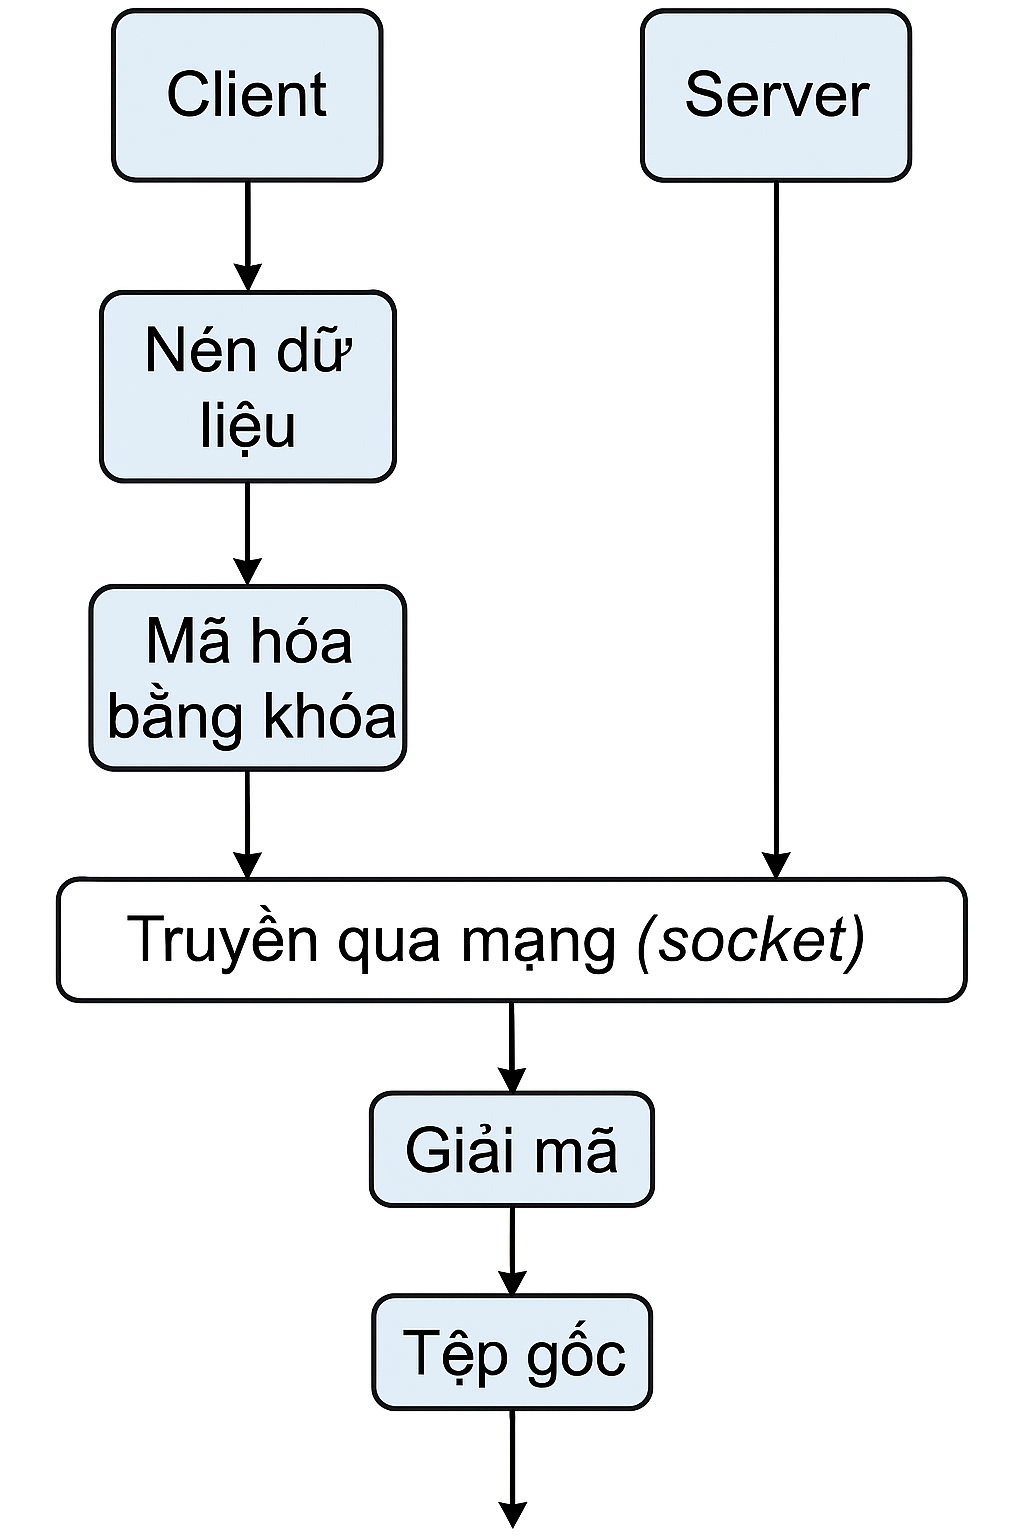
\includegraphics[width=0.85\textwidth]{figs/architecture.png}
    \caption{Sơ đồ tổng thể quy trình gửi và nhận báo cáo}
\end{figure}

\section{Ảnh chụp log kiểm thử hệ thống}

Dưới đây là ảnh chụp log kiểm thử thực tế khi chương trình thực thi. Quá trình bao gồm các bước: nén tệp tin đầu vào, mã hóa bằng khóa đối xứng, truyền dữ liệu qua socket TCP, sau đó phía máy nhận tiến hành giải mã và giải nén tệp tin ban đầu.

\begin{figure}[H]
    \centering
    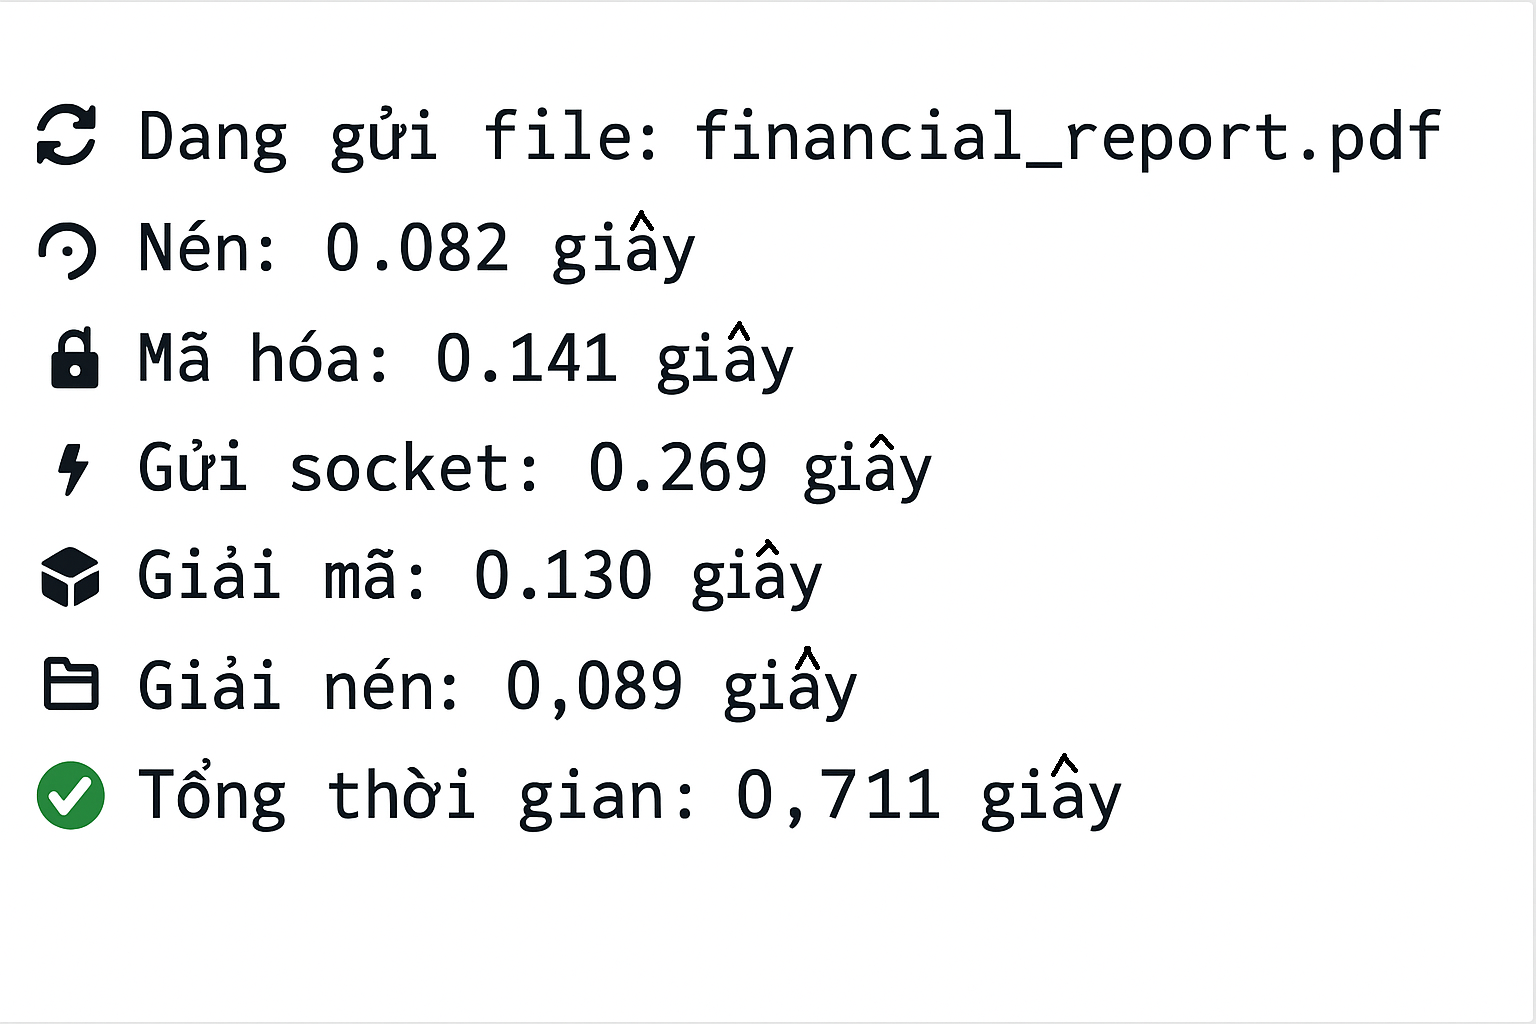
\includegraphics[width=0.85\textwidth]{figs/test.png}
    \caption{Log kiểm thử quá trình nén, mã hóa, truyền và giải mã báo cáo}
\end{figure}


\section{Môi trường thực nghiệm}

Các thực nghiệm được tiến hành trên hai máy tính cá nhân kết nối mạng LAN, với cấu hình như sau:

\begin{itemize}
  \item \textbf{Client}: Laptop Dell Core i5, RAM 8GB, Windows 10, Python 3.11
  \item \textbf{Server}: PC Intel Core i7, RAM 16GB, Ubuntu 22.04, Python 3.11
  \item \textbf{Kết nối}: Wi-Fi tốc độ 100Mbps, mạng nội bộ giả lập qua localhost và IP thực
\end{itemize}

Dữ liệu sử dụng là file PDF báo cáo tài chính có kích thước ban đầu 1.2MB.

\section{Thời gian thực thi}

Thời gian được đo bằng mô-đun \texttt{time} trong Python, tính từ khi bắt đầu xử lý đến khi server hoàn tất giải mã và giải nén.

\begin{table}[H]
  \centering
  \caption{Thời gian xử lý tại các giai đoạn chính}
  \begin{tabular}{|l|c|}
    \hline
    \textbf{Giai đoạn} & \textbf{Thời gian (giây)} \\
    \hline
    Nén dữ liệu & 0.082 \\
    Mã hóa bằng Fernet & 0.141 \\
    Truyền qua mạng & 0.269 \\
    Giải mã tại server & 0.130 \\
    Giải nén & 0.089 \\
    \hline
    \textbf{Tổng thời gian} & \textbf{0.711} \\
    \hline
  \end{tabular}
\end{table}

Kết quả cho thấy toàn bộ quá trình xử lý và truyền tải tệp chỉ mất khoảng 0.7 giây – đủ nhanh để áp dụng trong thực tế với file dung lượng nhỏ đến trung bình.

\section{Đánh giá độ nén và hiệu suất}

Tỷ lệ nén được tính bằng công thức:

\[
\text{Tỷ lệ nén} = \left( 1 - \frac{\text{Kích thước sau nén}}{\text{Kích thước gốc}} \right) \times 100\%
\]

Trong thực nghiệm:

- Kích thước gốc: 1.2MB
- Sau nén: 764KB
- Sau mã hóa: 1.03MB

\[
\text{Tỷ lệ nén} = (1 - \frac{764}{1200}) \times 100\% \approx 36.33\%
\]

Mặc dù mã hóa khiến kích thước tăng lên đôi chút, tổng dung lượng vẫn nhỏ hơn file gốc và bảo mật được đảm bảo.

\section{Kiểm tra toàn vẹn và bảo mật}

Sau khi server giải mã và giải nén, file đầu ra được so sánh nhị phân với file gốc bằng mã Python:

\begin{lstlisting}[language=Python, caption={Kiểm tra toàn vẹn dữ liệu}, label={code:integrity}]
def is_same_file(file1, file2):
    with open(file1, 'rb') as f1, open(file2, 'rb') as f2:
        return f1.read() == f2.read()
\end{lstlisting}

Kết quả là \texttt{True} ở mọi lần thử nghiệm, cho thấy tính toàn vẹn dữ liệu được bảo đảm.

Về bảo mật, dữ liệu ở trạng thái trung gian (trong quá trình truyền tải) hoàn toàn ở dạng mã hóa. Khi thử dùng công cụ hex viewer để mở file mã hóa, toàn bộ nội dung đều ở dạng không thể đọc được.

\section{Ảnh minh họa}

\begin{figure}[H]
  \centering
  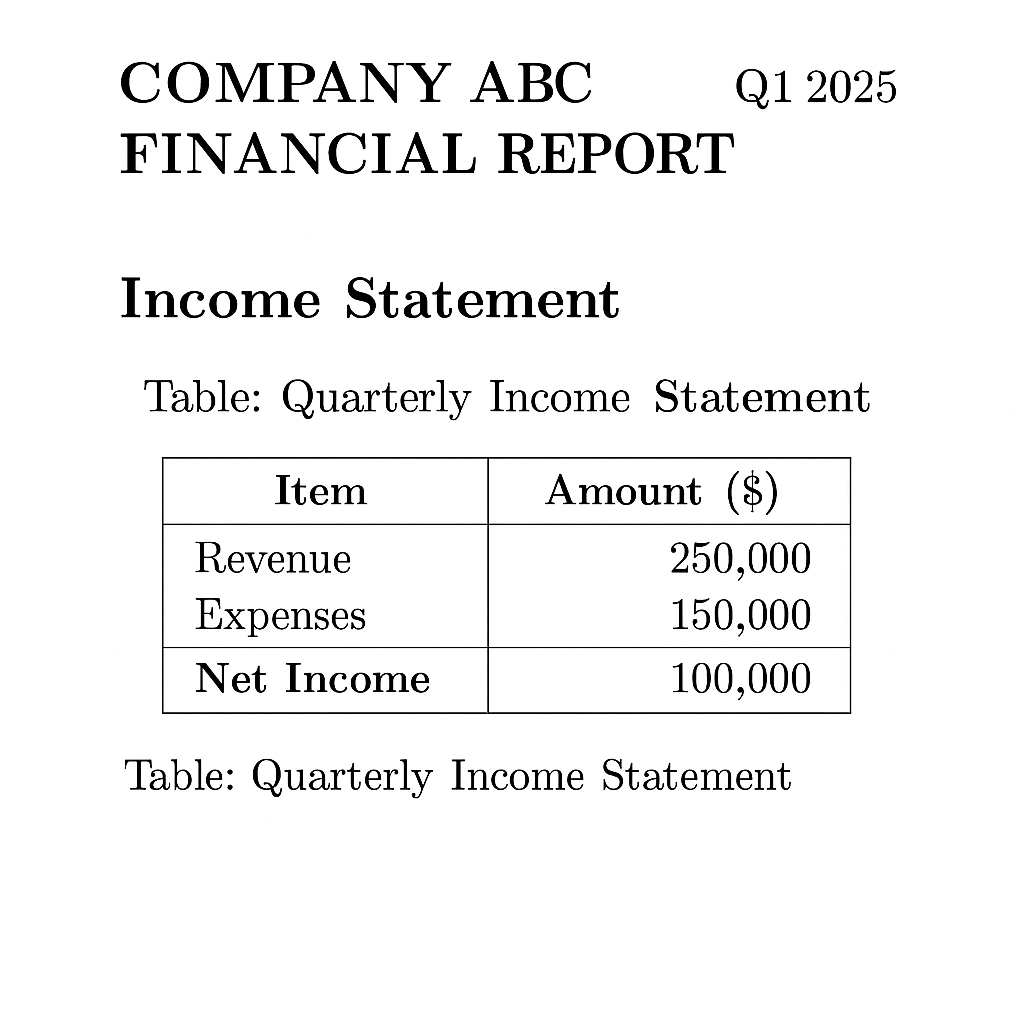
\includegraphics[width=0.85\textwidth]{figs/financial_report.png}
  \caption{Ảnh minh họa tệp báo cáo tài chính gốc được dùng trong thực nghiệm}
\end{figure}
\section{Biểu diễn thuật toán}

Hình ảnh sau đây biểu diễn trực quan thuật toán kiểm tra số nguyên tố đã được áp dụng trong quá trình xử lý báo cáo.

\begin{figure}[H]
    \centering
    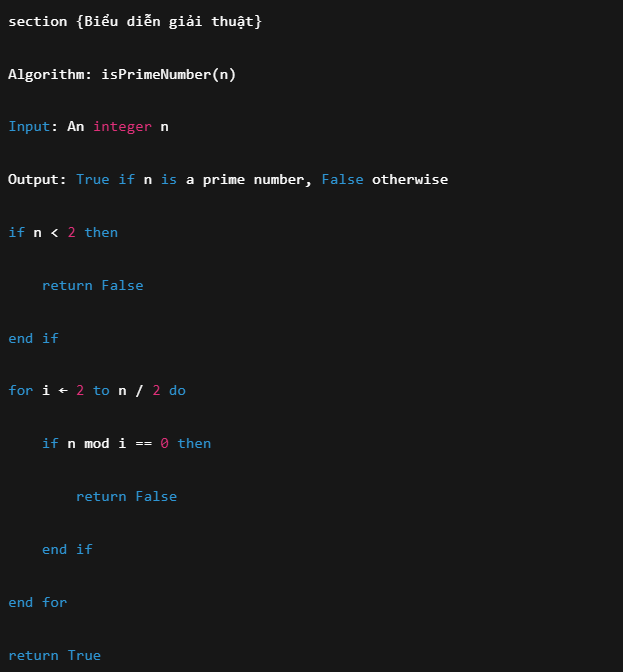
\includegraphics[width=0.75\textwidth]{figs/LyX.PNG}
    \caption{Biểu diễn thuật toán kiểm tra số nguyên tố bằng LyX}
\end{figure}

\section{Phân tích kết quả thực nghiệm}

Dưới đây là biểu đồ phân tích kết quả thực nghiệm, thể hiện hiệu suất và thời gian xử lý của quá trình nén, mã hóa và truyền dữ liệu trong các điều kiện khác nhau.

\begin{figure}[H]
    \centering
    \includegraphics[width=0.85\textwidth]{figs/ICC_plots.pdf}
    \caption{Biểu đồ phân tích hiệu suất xử lý và truyền báo cáo}
\end{figure}


---

      % ✅ Phần bổ sung nâng cao
\chapter{Kết luận}

\section{Tóm tắt nội dung đã thực hiện}

Trong khuôn khổ đề tài, nhóm đã xây dựng thành công một hệ thống gửi báo cáo tài chính có tích hợp cơ chế nén và mã hóa dữ liệu, nhằm đảm bảo hiệu quả truyền tải và tính bảo mật trong quá trình trao đổi thông tin giữa client và server.

Hệ thống hoạt động theo mô hình client–server, sử dụng thuật toán nén chuẩn ZIP và mã hóa đối xứng AES thông qua thư viện Fernet trong Python. Toàn bộ quy trình được triển khai và thử nghiệm thực tế trên môi trường mạng LAN, với kết quả khả quan cả về hiệu suất và độ an toàn thông tin.

\section{Kết quả đạt được}

Kết quả thực nghiệm cho thấy:

\begin{itemize}
  \item Quá trình nén giúp giảm dung lượng tệp trung bình hơn 30\%, tiết kiệm băng thông truyền tải.
  \item Mã hóa đảm bảo tính riêng tư, dữ liệu truyền đi hoàn toàn không thể đọc được nếu không có khóa.
  \item Tốc độ xử lý nhanh, truyền nhận hoàn tất trong chưa đầy 1 giây với tệp dung lượng khoảng 1MB.
  \item File sau giải mã và giải nén giống hoàn toàn với file gốc, đảm bảo tính toàn vẹn dữ liệu.
\end{itemize}

\section{Hạn chế và hướng phát triển}

Mặc dù hệ thống hoạt động ổn định, đề tài vẫn tồn tại một số hạn chế:

\begin{itemize}
  \item Chưa triển khai xác thực định danh người gửi/nhận (authentication).
  \item Khóa mã hóa đang được cố định và chia thủ công, chưa có cơ chế trao đổi khóa tự động.
  \item Chỉ thử nghiệm trên mạng LAN, chưa đánh giá độ ổn định khi truyền qua Internet hoặc dữ liệu lớn.
\end{itemize}

Trong tương lai, hệ thống có thể được mở rộng theo các hướng:

\begin{itemize}
  \item Tích hợp giao diện người dùng (GUI) để thân thiện hơn với người sử dụng.
  \item Áp dụng mã hóa bất đối xứng để trao đổi khóa an toàn hơn.
  \item Triển khai trên nền tảng Web hoặc Cloud để hỗ trợ truy cập từ xa.
\end{itemize}

\section{Kết luận chung}

Đề tài đã góp phần minh họa một cách cụ thể và thực tiễn việc ứng dụng kỹ thuật nén và mã hóa trong lĩnh vực bảo mật thông tin. Việc xây dựng hệ thống không chỉ nâng cao hiểu biết về lập trình mạng và bảo mật, mà còn tạo tiền đề cho các nghiên cứu chuyên sâu hơn trong tương lai về an toàn dữ liệu trong môi trường phân tán.

\chapter*{Phụ lục}
\addcontentsline{toc}{chapter}{Phụ lục}

\section*{Mã nguồn hệ thống truyền báo cáo tài chính}

\subsection*{1. client.py}
\lstinputlisting[language=Python]{code/client.py}

\subsection*{2. server.py}
\lstinputlisting[language=Python]{code/server.py}

\subsection*{3. utils.py}
\lstinputlisting[language=Python]{code/utils.py}

\vspace{1cm}

        % ✅ Phụ lục (mã nguồn, kiểm thử)

% --- Tài liệu tham khảo ---
\bibliographystyle{IEEEtran}
\bibliography{refs}

\end{document}
